%%%%%%%%%%%%%%%%%%%%%%%%%%%%%%%%%%%%%%%%%%%%%%%%%%%%%%%%%%%%%%%%%%%%%%%%%%%%%%%%%%%%%
% Machine Learning in Monitoring
%
% 1. Anomaly detection
%  - Adaptive using classifier updates
% 2. Alarm management
%  - Adaptive using RL
% 
%%%%%%%%%%%%%%%%%%%%%%%%%%%%%%%%%%%%%%%%%%%%%%%%%%%%%%%%%%%%%%%%%%%%%%%%%%%%%%%%%%%

ML prediction applications are effective complements to existing infrastructure in the process industry through soft sensors, state estimation, and forecasting. However, they are limited in applications regarding safety and risk management.  In the process industry, safety is upheld as the greatest \textit{value}; investing in a successful safety system is just good business.  

\begin{quote}
    "Safety is a \textbf{value}, not a priority.  Priorities change, but company values never do." \\
    --- Rex Tillerson, ex-CEO of ExxonMobil
\end{quote}

Decades ago, process safety investments are frowned upon by management due to its high costs and \textit{invisible} returns. In fact, construction workers used to cheer when project supervisors announced that \textit{only} 20 deaths will incur for this project---an event completely unacceptable in today's standards. Indeed, a perfect safety and risk management system results in \textit{no change} in day-to-day activities because all the incidents are proactively mitigated. As such, it is incredibly easy to become complacent towards risk management. However, if safety takes a back seat, the occurrence of the next incident is not a matter of if, its a matter of \textit{when}. Therefore, safety must be proactively (not reactively) managed to safeguard people, the environment, company assets, and production capabilities in terms of physical equipment and the social license to operate. Here, ML can be leveraged to proactively monitor process systems and create an additional layer of safety. In this chapter, ML algorithms will be applied to detect and predict equipment failures, process abnormalities, process variability and also perform alarm management. Through these applications, ML will be used to create multi-variate alarm systems that explore multi-variable interaction effects and gives fewer false alarms. Additionally, a new alarm management system that specifically tackles alarm flood scenarios will be introduced.  The objectives of this system are twofold: 1) Reduce sheer number of alarms during a flooding scenario; 2) identify the most important alarms so operators can prioritize safety critical alarms.

This chapter is organized as follows: Section 1 introduces data pre-processing methods for anomaly detection/prediction applications where the data is heavily imbalanced.  Section 2 introduces the anomaly detection and prediction algorithms and section 3 concludes this chapter with an introduction to a novel approach for alarm management.

The main contributions of this chapter are the data pre-processing methods used to prepare data sets for anomaly detection/prediction.  Additionally, it was shown that using synthetic data was able to enhance accuracy.  Lastly, a novel alarm management approach based on reinforcement learning was introduced to filter nuisance alarms and sort alarms based on their priority.  




Heavily unbalanced data:
- SMOTE, ADASYN, Breaking time down into smaller segments and increasing sampling rate

\section{Data Pre-processing for Monitoring}
Data containing anomalous and/or incident events are extremely rare---thankfully---in the process industry. \begin{quote}
    Anomaly or anomalous activity: An abnormal or unexpected event given other variables (often multivariate).  For example, a person walking in a t-shirt when it is -$\ang{30}$ C outside.
\end{quote}

In fact, it is not uncommon to have just one incident in a data set containing hundreds of thousands of records.  Under such circumstances, building ML models to identify incidents is extremely difficult.  Remember, ML models are nothing more than statistical models with training formulated in an incremental updating fashion. In the scenario where the training data set contains 999,999 non-anomalous activities with 1 anomalous activity, the model will simply learn to return non-anomalous for all inputs; such a model would still achieve 99.9999\% accuracy on the training data!  When a human is provided with this data set, the human would instead focus most of its attention on the one anomalous activity, studying how it is different from all the other points.  A \textit{tabula rasa} machine is simply not equipped with such cognitive abilities, and will treat every data point equally; however, humans can artificially provide cognition to the machine.

\subsection{Data Prep for Anomaly Detection}
Anomaly \textit{detection} tasks are quite simple compared to anomaly \textit{prediction} tasks that will be discussed later on in this section. In anomaly detection, the model simply has to classify if there is an anomaly at current time. For example, given some states of a reactor, is the output temperature anomalous? That is, is the measured output temperature expected given the states?  Of course, such questions are difficult for humans to answer, especially in multi-variate environments; however, such questions can easily be answered by machines. Unfortunately, the events that are of interest to us (anomalies) are, often times, significantly more rare compared to normal process data. Hence, the leading reason for poor model performance in imbalanced data sets (i.e., distribution of different classes are vastly different) is the \textit{imbalanced} nature.  There exists two traditional ways to tackle the data imbalance issue: \textbf{undersampling} and \textbf{oversampling}.  Objectively, both methods aim to re-balance the data set so that the positive and negative data are in harmony.

A visual description of undersampling and oversampling is shown in Figure \ref{fig:03under_over_sampling}. In undersampling, 

\begin{figure}[H]
    \centering
    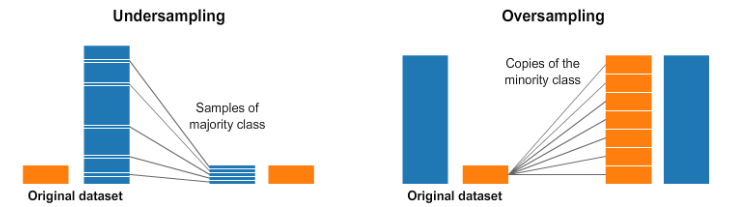
\includegraphics[width=0.8\textwidth]{images/ch3/over_and_undersampling.jpeg}
    \caption{A visual representation of undersampling (left) and oversampling (right). Original image from Kaggle.}
    \label{fig:03under_over_sampling}
\end{figure}

\subsection{Data Prep. for Anomaly Prediction}

\subsection{Synthetic Data Generation}


\section{Anomaly detection and prediction}


The model structure for logistic regression is given as:
\begin{equation}
    \hat{y} = \frac{1}{1 + e^{-(W_1^Tx + W_2^Tu + b)}}
    \label{eq:02LogS}
\end{equation}
where $e$ denotes the exponential operator.

- Measure process variability?

\subsection{Deep Learning Classification and Prediction}

\subsection{Explanability}
- Explanability through weights, through importance sampling

\section{Alarm Management}

\subsection{Alarm Prioritization}

\subsection{Alarm Reduction}
